\documentclass{article}

\usepackage[utf8]{inputenc}  
\usepackage[T1]{fontenc}    
\usepackage{graphicx}
\usepackage{caption}

\begin{document}

\title{Sur les méthodes de résolution du Problème de transport à la demande}
\author{Adegnandjou Eddy, Walid Yahia Mahammed}
\date{\today}
\maketitle

\newpage

\paragraph{Optimisation combinatoire}
L'optimisation combinatoire est une branche de la programmation mathématique née pour répondre aux besoins de plusieurs domaines dont l'informatique. L'optimisation combinatoire s'intéresse à des problèmes pour lesquelles il y a souvent un très grand nombre de solutions, qu'il n'est pas possible de d'explorer de façon explicite pour déterminer un meilleur choix.

\section{Classification des méthodes d'optimisation}
\paragraph{}
Nous étudions ici la classification des méthodes d'optimisation.
\begin{figure}[h]
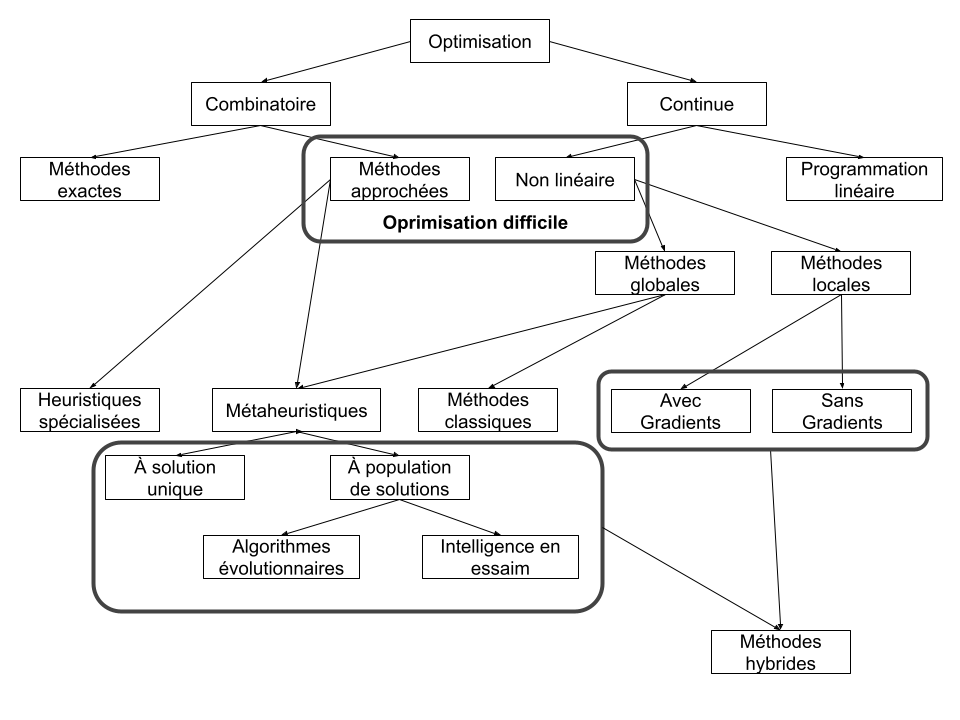
\includegraphics[scale=0.4]{images/classification-des-methodes-doptimisation.png}
\caption{Classification des méthodes d'optimisation \cite{12-dreo}}
\end{figure}
\paragraph{Contexte}
Les récents progrès technologiques ont fait naître de nouveaux besoins en transport. Pour répondre à ces besoins, certains services de transport innovants tels que les véhicules intelligentes ont vu le jour, ils s'inscrivent dans le cadre du transport à la demande et font face au défis de l'organisation du transport.

\paragraph{Positionnement}
La caractéristique principale du transport à la demande est la réactivité du système de transport à des demandes en temps réel. La différence par rapport au bus est qu'il n'y a pas d'itinéraire et d'horaire figés, contrairement au taxi le transport à la demande n'est pas à vocation individuel mais collectif. Ces deux aspects offrent une flexibilité  intéressante à l'utilisateur de ce type de transport. Si on élève le niveau d'abstraction, un tel système peut être assimilé à un réseau de transport où les requêtes de transport sont caractérisés par une origine, une destination, le nombre de passagers est les heures de passage. D'autres informations intéressantes peuvent être identifiées: un système déterministe selon qu'on peut prévoir les demandes de transport ou stochastique sinon. D'un point de vue économique, les requêtes de transport correspondent à la demande alors que les véhicules chargés d'effectuer le trajet correspond à l'offre. 

\paragraph{Problèmes techniques}
Les défis techniques que pose l'organisation du transport à la demande sont de l'ordre de l'algorithmique, de la modélisation et concernent aussi le mode de transport. Algorithmiquement, le DARP se décompose trois problèmes. Premièrement un problème d'affectation ou clustering problem où il est question d'affecter le véhicule adéquat pour répondre à une requête donnée. Deuxièmement il peut être abordé comme un problème de séquencement ou routing problem. Le troisième problème auquel se rapporte un cette organisation est l'horodatage ou sheduling problem. Le séquencement et l'horodatage peuvent être étudier ensemble sous forme de problème d'ordonnancement. On parle de problématique d'ordonnancement en présence de contraintes temporelles. Le contexte des problèmes techniques peut être statique ou dynamique. Dans le mode statique, le plan de transport est établi avant d'effectuer le trajet, toutes les informations sur les différentes requêtes sont connues et utilisées pour construire l'itinéraire à suivre par les véhicules. Notons que cela diffère quand même du plan de bus dont l'itinéraire est figé. Parafais \cite{Parafais} pose une frontière entre le routage de véhicule statique et dynamique en fonction de l'évolution en temps réel des données d'entrée pour planifier la tournée.

\paragraph{Algorithmique et complexité}
La complexité permet de mieux caractériser les difficultés rencontrées par les méthodes de résolution pour déterminer une solution à un problème d'optimisation combinatoire.

\paragraph{État de l'art}
Une fenêtre de temps est la période de temps spécifiée par une date au plus tôt et une date au plus tard durant laquelle une demande de chargement ou de déchargement est satisfaite. Elle permet d'indiquer des contraintes de temps, liées aux véhicules ou aux clients. Dans le cas où un véhicule arrive avant sa fenêtre de temps, une attente est crée et cela affecte la qualité de service considéré dans le DARP.

\paragraph{Heuristiques}
Les méthodes heuristiques ne garantissent pas l'optimalité de la solution, mais permettent d'obtenir un résultat de bonne qualité au bout d'un temps raisonnable. Il existe trois catégories d'heuristiques pour le DARP avec plusieurs véhicules. Il s'agit du cluster-first route second, l'amélioration locale et les procédures d'insertion \cite{13}. 

	Le PDTW est structurellement très proche du DARP. Ainsi, plusieurs méthodes de résolution du DARP sont une adaptation des méthodes de résolution du PDTW. De même, le cluster-first route second provient du VRP et est une adaptation au DARP. Il décompose le problème en un problème de partitionnement où il est question d'affecter un groupe d'usagers au véhicule qui se chargera de les transporter; puis un problème d'élaboration des tournées. Baugh et al. (1998) \cite{10-113} résolvent le problème de partitionnement avec une méta-heuristique de type \textbf{recuit simulé} et l'élaboration des tournées avec une heuristique basée sur la recherche des \textbf{plus proches voisins}. Une \textbf{recherche taboue} est également utilisée pour le DARP statique par Cordeau et Laporte (2003) \cite{10-77}. Une méthode de \textbf{recherche locale} a été proposée par Van Der Bruggen et al. (1993) \cite{10-72} pour le problème de chargement et déchargement avec un seul véhicule et des fenêtres de temps.
	
	Plusieurs procédures pour améliorer les solutions obtenues par une heuristique d'insertion sont étudiés par Toth et Vigo (1996) \cite{10-116}.
	
	Les  heuristiques d'insertion sont rapides, faciles à implémenter. Elles peuvent être étendues pour prendre en compte de nouvelles contraintes \cite{10-123}, ce qui est particulièrement convenable pour un problème fortement contraint tel que le DARP. On a l'insertion partielle, exhaustive, avec trie des demandes puis avec réparation (forte).

	Xiagang Zhao \cite{13} propose deux heuristiques gloutonnes basées sur la technique d'insertion pour le DARP: une heuristique d'insertion partielle et une heuristique d'insertion exhaustive qui sont comparés à l'\textbf{algorithme génétique} et la recherche taboue. Ces travaux montrent que les deux procédures d'insertion donnent des résultats de bonne qualité qui assurent une meilleure qualité de services. Il présente également une heuristique mémoire basée sur la technique d'insertion et la propagation de contraintes. Puis une recherche locale avec usage limitée de la procédure SPLIT est effectuée pour améliorer le résultat de l'heuristique d'insertion. Une méthode de résolution du DARP multi-objectif basée sur la métaheuristique \textbf{ELS} utilisant le \textbf{front de Pareto} \cite{13} permet d'atteindre des résultats pouvant rivaliser avec la recherche taboue et l'algorithme génétique. Les heuristiques: basique, mémoire, avec recherche arborescente sont adaptées pour traiter le DARP avec contraintes financières, un problème jamais traité auparavant.
\section{Problème du voyageur de commerce}

\section{Problème de tournée de véhicule}

\section{Programme linéaire}

\section{Programmation/optimisation linéaire en nombres entiers}

\section{Problème du transport à la demande}
\paragraph{}
De sa dénomination anglaise DARP ()


\section{Méthode exacte}


\section{Mat-heuristique}

\section{Caractérisation de l'offre}

\section{Caractérisation de la demande}

\section{Problème de dégénérescence}

\section{Solution optimale du primal/dual}

\section{Relaxation linéaire}
La relaxation d'un problème consiste à l'étudier dans un espace plus étendu dont on dispose de suffisamment d'outils théoriques pour mieux l'appréhender. Cette manœuvre est utile en particulier pour la résolution du problème principal de la méthode de génération de colonne présentée dans le second chapitre. La résolution de la relaxation d'un problème peut être utile à sa propre résolution. Ceci a été démontré par Karmarkar \cite{Karmarkar} en se basant sur un problème de programmation quadratique.

\section{Introduction}

\paragraph{}
La synthèse bibliographique effectuée dans ce rapport porte sur les méthodes de résolution du problème du transport à la demande (TAD). L'objectif de cette étude est d'aborder ce thème sous différents angles de vue, afin d'en cerner efficacement le contour et de donner une orientation future à la rédaction de notre mémoire. Nous y arrivons à travers une description synthétique des idées que suscite un questionnement systématique suivie d'une analyse critique. Ensuite nous positionnons notre thème par rapport à d'autres travaux de recherche avant de conclure pour énoncer les ressources pertinentes de la littérature scientifique utilisées.


\section{Description synthétique des idées développées}

\paragraph{}
Plus anciennement appelé Bus à la demande ou Minibus à la demande, le transport à la demande consiste à allier la flexibilité dans le choix des endroits parcourus et l’accessibilité du transport en terme de coût. Il se veut adapté à des contextes totalement hétérogènes tant en interne qu’à une échelle plus globale de géants réseaux routiers. Sa particularité est qu’il n’est activé que lorsqu’un potentiel usager en fait la demande.

\paragraph{}
D'un point de vue purement scientifique, le problème du transport à la demande se rapporte à la détermination d'un chemin ou circuit au sein d'un réseau de transport en respectant certains critères définis selon la demande et mathématiquement modélisés. Ce chemin est obtenu à l'aide d'outils algorithmiques permettant de résoudre le problème et choisis selon les objectifs visés: il peut s'agir de satisfaire des exigences de temps, de coût ou de qualités de services.

\paragraph{}
Il existe plusieurs approches de résolution des TAD. Ces méthodes peuvent être classées en trois catégories. Premièrement, on distingue les méthodes de résolution exactes qui garantissent fiabilité des résultats avec des solutions optimales. Une deuxième catégorie concerne les méthodes de résolution approchées qui ont pour objectif de résoudre le problème efficacement. Finalement, nous avons les méthodes de résolution basées sur les systèmes multi-agents qui permettent de gérer la complexité dans la résolution.

\paragraph{}
Le transport à la demande répond à une problématique d’actualité: la forte mobilité pour laquelle les moyens existants tels que le bus, le taxi et même la voiture personnelle, traditionnellement utilisés se révèlent trop contraignants pour les usagers. TAD concerne essentiellement toute personne intervenant dans un réseau routier et qui utilise un moyen de transport pour se déplacer.

\paragraph{}
Le transport à la demande bien qu'indépendant d'un contexte géographique particulier est assez développé dans certains pays d'Europe et très évolué dans les zones les plus urbanisés des États-Unis. Il se développe aussi dans d'autres régions du monde.

\paragraph{}
Le TAD est issu d'un problème plus ancien: le problème du voyageur de commerce. Ce dernier a ensuite été généralisé en problème de tournées de véhicules dont l'une des variantes est le problème du transport à la demande.

\paragraph{}
Le transport à la demande utilise les moyens de déplacement en commun comme le bus et fonctionne d'une manière assez singulière. Le système n'est déclenché que s'il y a au moins une demande d'un usager. Il utilise un réseau routier et tente de s'adapter aux préférences des utilisateurs.

\paragraph{}
Pour résoudre le problème de transport à la demande, l'approche intuitive serait d'explorer de façon exhaustive l'ensemble des solutions envisageables puis de les évaluer afin de choisir celle qui correspond au mieux à la situation. Cependant, cette démarche peut s'avérer très coûteuse, sinon irréaliste dans un délai limité. Il convient donc d'utiliser des moyens appropriés pour obtenir le chemin recherché.


\section{Analyse critique des idées, forces et faiblesses}

\paragraph{}
Les méthodes de résolution exactes permettent de mener une étude suffisamment précise et fiable. Cependant elles ont du mal à gérer la complexité des problèmes de taille considérable. Quant aux méthodes de résolution approchées, elle sont utiles pour trouver rapidement une solution admissible, même si l'optimalité de la solution trouvée n'est pas la meilleure. Enfin, les méthodes de résolution basées sur les systèmes multi-agents permettent de gérer la complexité du problème en se basant sur des algorithmes d'intelligence artificielle. Il peut être utile de se servir d'un type spécifique de méthode ou d'en combiner certaines, selon le cas.

\section{Positionnement du TAD par rapport aux autres travaux}

\paragraph{}
Les problèmes de tournée concernent l'organisation de la mobilité étudié par l'optimisation combinatoire et la recherche opérationnelle.

\paragraph{}
Le TAD fait parti de la famille des problèmes de tournées de véhicule (VRP), dont le plus populaire est celui du voyageur de commerce TSP. Plusieurs travaux sur le TSP ont conduit à l'élaboration de méthodes de résolution en optimisation combinatoire et en recherche opérationnelle(\cite{Nobody06}). Pour résoudre les problème de cette catégorie, les graphes sont un excellent outil de modélisation. En théorie des graphes, le TAD se rapproche du problème de recherche d'un circuit hamiltonien.

\paragraph{}
Le problème du transport est tout d'abord un problème d'optimisation combinatoire. Il appartient à la catégorie des problèmes d’optimisation combinatoire NP-Difficile, NP-complet et peut être mono-objectif ou multi-objectif. Il intéresse de ce fait la communauté de la recherche opérationnelle d'une part. D'autre part, les sociologues s'interrogent sur les raisons qui motivent un important flux de transport ainsi que l'impact de ce fait sur la société. Les géographes quant-à eux s'intéressent à l'interaction entre les territoires et les réseaux.


\section{Conclusion}

Le problème de transport à la demande est un problème d'actualité dont la résolution peut bénéficier des récentes avancées scientifiques d'autres domaines tels que l'intelligence artificielle. Considérant que l'étude bibliographique est un processus évolutif nécessitant une veille bibliographique, les résultats présentés dans ce rapport constituent une base de travail qui sera progressivement enrichie tout au long de la rédaction du mémoire. Ils permettront de poursuivre la synthèse bibliographique en explorant le réseau de citations, les références des publications pertinentes sur les méthodes de résolution du transport à la demande.

\section{Méthode de génération des colonnes}
La méthode de génération des colonnes se base sur l'idée que toutes les variables ne sont pas forcément utiles pour trouver la solution optimale, elle peut être utilisée sous forme de méthode exacte ou en tant qu'heuristique. C'est une méthode itérative où une colonne correspond à une variable. Le problème initial est donc traité sous forme de problème maître alors qu'un problème esclave se charge de générer les nouvelles variables à considérer dans chaque itération en considérant les contraintes de faisabilité. Cette méthode utilise la solution duale et les coûts réduits. Puisqu'on a besoin des variables duales, la génération de colonnes ne fonctionne que sur les problèmes en nombre réel. La méthode de simplexe tout comme l'algorithme du point intérieur peut être utilisée à ce niveau pour résoudre le problème maître car il permet d'obtenir une solution optimale du primal et du dual. Cette opération se déroule avant de s'intéresser au problème esclave, au sein d'une même itération. [Schéma récapitulatif] Même si elle est très efficace en pratique, la méthode de simplexe peut dans le pire des cas conduire à une complexité exponentielle \cite{Simplex}.


\bibliographystyle{plain}
\bibliography{my}

\paragraph{}
Thierry Garaix.Étude et résolution exacte de problèmes de transport à la demande avec qualité de service. Modélisation et simulation. Université d’Avignon, 2007. Français. tel-00534894

Anas Malas. Contributions à la résolution du transport à la demande fondées sur les systèmes multi-agents. Intelligence artificielle [cs.AI]. Normandie Université, 2017. Français. NNT : 2017NORMIR07. tel-01661358v2


\end{document}